Tras haber expuesto las motivaciones y el contexto en el que se engloba este proyecto de fin de grado, en este capítulo daremos una explicación más detallada del problema que se
intenta resolver y los pasos dados para conseguirlo.


\section{Descripción del problema}
\label{sec:descripcion del problema}

En la actualidad la robótica está en nuestro alrededor en todo momento, debido a las nuevas tecnologías y al abaratamiento de costes se encuentra en pleno auge. A pesar de que convivimos a diario con ella por lo general sigue siendo un enigma para la mayoría de las personas.

No es menos cierto que existe una enorme complejidad que requiere de un alto conocimiento de las tecnologías implicadas tras la configuración de un robot, y es esta barrera la que queremos eliminar.

Con este proyecto buscamos el acercamiento de la robótica a un público con escasos conocimientos técnicos, simplificando al máximo toda la complejidad que existe tras la programación de un robot, hasta el punto que sea usada por niños para el aprendizaje, haciendo el mundo de la robótica más cercano y más atractivo a ojos de aquellos que serán el futuro de ésta.

Esto lo conseguimos creando un nexo entre un lenguaje de programación visual mediante bloques, para esto hacemos uso de \textit{Scratch}, y la programación de robots en Python. Con \textit{Scratch4Robots} conseguimos que partiendo de un lenguaje fácil e intuitivo, basado en el apilamiento de bloques funcionales de código, la traducción a código Python completamente funcional. Creando unos bloques con funcionalidad dirigida a robots en especifico conseguimos que esta traducción pueda ser aplicada a robots.    

\section{Requisitos}
\label{sec:requisitos}

Para cumplir los objetivos marcados de forma satisfactoria, debemos además satisfacer
los siguientes requisitos:

\begin{itemize}
\item El desarrollo deberá ser autocontenido en lo que sea posible, esto quiere decir que todas las librerías y dependencias de nuestra herramienta deberán estar contenidas en su interior. La programación se realizará en el
lenguaje Python.
\item El software desarrollado deberá ser compatible con Ubuntu 16.04, ROS-kinetic y Scratch 2.0 serán los únicos elementos indispensables para el correcto funcionamiento de nuestra herramienta.
\item Todos los componentes desarrollados deberán ser compatibles tanto trabajando en entornos simulados, como usando robots reales, esto se consigue usando todas las abstracciones de las que nos provee JdeRobots, totalmente testadas en robots reales.
\end{itemize}



\section{Metdología de trabajo}
\label{sec:metodologia}

Dada la naturaleza del proyecto, y al igual que en cualquier otro proyecto de software, es necesario el uso de un modelo que defina el ciclo de vida de la aplicación. Para el desarrollo de este proyecto hemos decidido adoptar el modelo de desarrollo en espiral.
TODO BIBLIOGRAFIA
El modelo en espiral consiste en una serie de ciclos que se repiten en forma de
bucle, cada ciclo representa un conjunto de actividades. Las actividades no están
prefijadas \textit{a priori}, sino que se eligen en función de las realizadas previamente. Estos
ciclos se irán ejecutando hasta que la aplicación sea aceptada y no requiera otro
ciclo. Este modelo, definido por Barry Boehm en 1986, se basa en una espiral en la que cada iteración representa un conjunto de actividades.Estas actividades no tienen prioridad, se elegirá en la fase de análisis de riesgos. Así, cada iteración está dividida en las siguientes actividades:

\begin{itemize}
\item Determinar objetivos: en esta actividad se definirá el objetivo de la iteración actual. Siguiendo este
modelo el objetivo final del proyecto se divide en sub-objetivos.
\item Análisis de riesgo: en esta actividad, se lleva a cabo varios estudios con el propósito de conocer las
posibles amenazas o eventos no deseados que se puedan producir en el objetivo actual.
\item Desarrollar y probar: llegados a este punto será necesario la verificación del correcto funcionamiento realizado en la iteración para subsanar los errores y que estos no prosigan en las siguientes iteraciones.
\item Planificación: en esta actividad se revisarán las fases anteriores para determinar si se debería continuar.
\end{itemize}

\begin{figure}[h]
    \centering
    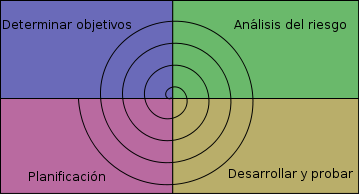
\includegraphics[width=0.75\textwidth]{img/metodologia_espiral}
    \caption{Desarrollo en espiral}
    \label{fig:espira}
\end{figure}

Para materializar estas actividades e iteraciones mantuvimos reuniones semanales durante todo el desarrollo del trabajo. De este modo, cada semana marcábamos un nuevo subobjetivo. Si el anterior se había completado, planificábamos el siguiente. Si por el contrario, no sé había completado, ahondábamos en el objetivo actual para corregir los errores o volver a planificarlo.

Todo el código fuente generado se mantuvo en un repositorio con un sistema de control de versiones (SVN), \textit{Git} en nuestro caso, accesible desde internet[TODO enlace a git].

De este modo el tutor y cualquier otra persona interesada tiene acceso en cualquier momento al código, además nos apoyamos del sistema de apertura de \textit{issues} en el repositorio remoto \textit{Git} para cada implementación que se necesitaba desarrollar para la mejora del proyecto. 

\section{Plan de trabajo}
\label{sec:plan}

Simplificaremos la labor a desarrollar en varios puntos:
\begin{itemize}
\item \textbf{Familiarización con el entorno software}: JdeRobot es la plataforma de desarrollo principal utilizada en la mayoría de proyectos realizados en el departamento de robótica
de la URJC. El objetivo principal de esta fase es aprender a utilizar este software, sus
componentes y sus drivers para más adelante utilizarlos como parte de nuestro proyecto.
Como parte del aprendizaje, se desarrolla una herramienta externa al core principal pero que usa de librerías y recursos de ella.
\item \textbf{Estudio de KURT}: Librería que nos permite obtener toda la información necesaria de un proyecto Scratch, conocimiento de su API y su funcionamiento interno para saber qué podemos llegar a obtener y como usar esa información para proporcionar una traducción robusta al lenguaje Python.
\item \textbf{Desarrollo de funcionalidades}: Aumentamos el número de bloques robóticos própios que podremos usar en Scratch, esto es desarrollar la lógica detrás de cada bloque, todo programado en python y la integración de estos bloques con Scratch. Dividimos los bloques entre aptos para drones y robots con ruedas. Estos bloques deben tener una funcionalidad muy específica y funcionar en armonía con el resto, tanto los propios de la aplicación Scratch como los nuevos bloques generados por nosotros propios de aplicaciones robóticas.
\item \textbf{Facilitar el uso de la herramienta}: Haciendo el uso de la herramienta lo más intuitiva posible, mejorando scripts de lanzamiento y de generación de código. Creando ejemplos autocontenidos para una rápida demostración de la potencia de la herramienta. Generando tutoriales tanto escritos como con vídeo para evitar confusiones.
\item \textbf{Integración}: La parte sin duda más compleja del desarrollo ya que se busca que nuestra aplicación sea fácilmente instalable en cualquier entorno y con la mayor facilidad posible, únicamente necesitando las dependencias que hemos comentado con anterioridad. Teniendo en cuenta que debe ser fácilmente usada por personas con pocos conocimientos técnicos.


\end{itemize}
